\chapter[Summary and Proposed Work]{Summary and Proposed Work}

\section{Summary}
The need of proposed work had been shown by a summary of the 
current state of the art of \glspl{MSR} online reprocessing 
simulator capabilities. The literature review in Chapter 2 
concluded that most \gls{MSR} depletion simulators typically 
assume ideal (rather than realistically constrained) poisons 
removal rates (e.g., 100\% of target poison mass is extracted) 
for the nuclear system performance modeling. The Python 
toolkit, SaltProc, directly coupled with SERPENT 2 Monte Carlo Burnup 
code for liquid-fueled \gls{MSR} depletion simulation 
including realistic online reprocessing plant to be developed 
in this work. Proposed work will provide a currently unavailable 
tool for fuel composition evolution analysis in \gls{MSR} with 
an online reprocessing system involving multiple processes 
that vary in their extraction efficiencies and rates. Finally, 
the tool capabilities will be demonstrated for few promising 
\gls{MSR} designs including \gls{TAP}, 
\gls{MSBR}, \gls{MSFR} and validated against exist in the 
literature analysis.

 
\section{Proposed Work and Simulations}
A new SaltProc Python-based fuel cycle simulator, coupled with
the SERPENT 2 Monte Carlo code, incorporating user-parametrized 
components in the fuel salt processing system design will be 
developed and validated in three stages. A demonstration stage will implement 
an ‘no reprocessing’ \gls{MSR} structure which captures the 
fundamental code behavior of the components and integrated nuclear 
system model. On this stage obtained simulation results will be 
verified to SERPENT 2 results for stationary fuel salt which 
might be useful for debugging in early stage of tool development.
A base case stage will build upon the demonstration model by 
adding simple poisons removal with constant extraction efficiency 
and compensation fissile material feed and will be 
verified with ChemTriton results for unit cell and full-core 
geometry from recent \gls{ORNL} research 
\cite{betzler_two-dimensional_2016, betzler_assessment_2017}.
The final extension stage will build upon the base case by 
implementing extending physics and chemistry correlations for 
extraction efficiencies to capture impact of non-ideal 
removal rates in the reactor performance modeling. These 
stages will be completed withing a test-driven software 
development paradigm, will leverage unit tests and 
continuous integration for sustainable development. Finally, 
collected during these stages data will be organized and 
published in a \textit{.JSON} format data library for use 
with the SaltProc Python package.
\begin{figure}[ht!] % replace 't' with 'b' to force it to 
  \centering
  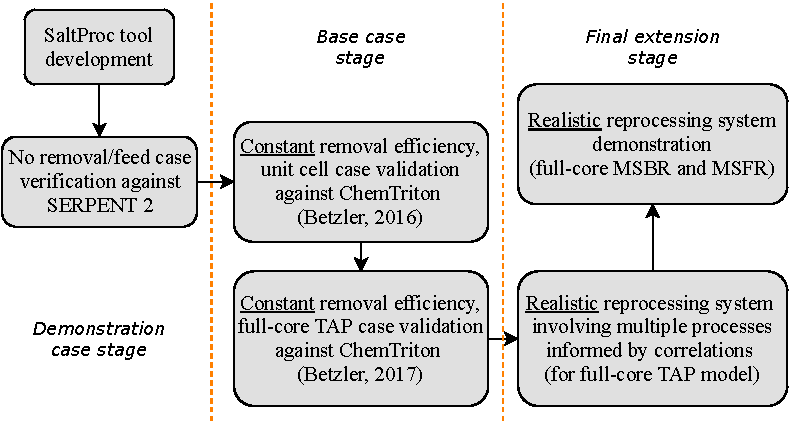
\includegraphics[width=\textwidth]{workflow_for_thesis.pdf} 
  \caption{Workflow for the simulations proposed in this work..}
  \label{fig:workflow}
\end{figure}

Additionally, sensitivity analysis for \gls{TAP} fuel processing 
system design will be performed to determine desirable ranges 
for principal system parameters. Particularly, inputs to the 
system model (e.g., components volumes, holdup capacities, helium 
bubble size, etc) will be sampled randomly from appropriate 
distributions to obtain results (e.g., fuel utilization) in the 
form of corresponding distributions. These data later can be used 
to formulate design requirements and safety margins for 
\gls{MSR}'s reprocessing system designers.

\subsection{Demonstration Case Development}
The proposed tool preliminary class structure and flowchart are 
described in detail in section~\ref{sec:tool_design}.
A first milestone in the development of this toolkit will be a 
principle demonstration of coupling with SERPENT 2 and 
information passing schemes. That is, no removals or feeds 
will be implemented in this demonstration stage. However, 
the components models will be developed in such way that 
they are capable of passing data about material (e.g., isotopic 
composition vector) via set of \textit{Processes} but this 
processing system will not actually modify \textit{MaterialFlow} 
(separation efficiency is to be set 0\%).

The demonstration will produce a complete but 'empty' processing 
model. It will allow to simulate \gls{MSR} system operation during 
longtime period and obtain resulting fuel salt isotopic composition. 
After that, the result will be verified against fuels salt 
composition obtained for the same depletion parameters and the 
core geometry with pure SEPRENT 2 code because this case does not 
introduce any online processing challenges.

At the subcomponent level, the demonstration will include information 
passing, bookkeeping, mass balance within and between the 
subcomponents. Information passing between subcomponents 
(\textit{Processes}) concerning nuclide concentration, mass flow rate 
and total volume in \textit{MaterialFlow} will be implemented and tested. 
A HDF5 output database structure will be defined and 
bookeeping for writing isotopic composition vector, simulation 
parameters and all relevant processing information.

This work will be developed with a test-driven development paradigm. 
Specifically, before any new functionality is implemented, a suite of 
tests is written which as closely define its expected behavior as 
possible. The code is then written with the goal of passing the test 
suite. In this way, the tool developed in this work is expected to be
comprehensively tested in parallel with its development.

Test problems will help comprehensively define and confirm each unit 
of the demonstration functionality. These problems will include very 
basic information passing tests as well as more challenging multiple 
components integration tests. Every unit of functionality
within the toolkit should be tested as an integral part of development.

When these unit test suite passes, validation efforts against results 
in the literature will take place to demonstrate that the complete 
processing system model behaves in agreement with previous research 
efforts. If it does not behave as expected, sensitivity analyses, 
model abstraction, and computational development will be iterated 
through until the model is validated.

\subsection{Base Case Development}
The next stage in this work will be the development of the base case. 
This will build upon the demonstration processing system model by 
implementing simplified physics for each of the subcomponents. This 
will include constant non-ideal extraction efficiency which is 
different for each target chemical element. Moreover, realistic 
model of \gls{TAP} reprocessing plant involving multiple 
processes (serial and parallel) will be implemented on this 
stage. 

Additional information such as void fraction, helium 
bubbles size and other component-specific users-defined 
parameters will be added to demonstration case model.
Also this will include non-zero fuel salt feed which 
compensate removed poisons mass loss in a primary loop.
This milestone will result in a processing system model capable of 
modeling various liquid-fueled \gls{MSR} with comprehensive 
online reprocessing system but with constant, defined at runtime 
separation efficiency.

Unit testing, verification and validation will occur in a manner 
very similar to the previous case. Unit tests will assess the 
performance of each extension functionality as well as their 
integrated behavior. Validation against exist results for \gls{TAP} 
obtained by ChemTriton \cite{betzler_two-dimensional_2016, 
betzler_molten_2017} will also be performed for confidence 
building.

Additionally, the base case model will be used to estimate 
effective 
multiplication factor ($k_{eff}$) dynamics for long-time 
depletion simulations. Particularly, it will demonstrate 
ability of \gls{TAP} system maintain critical state with 
fresh salt feed rate equal rate of loss 
of separated (with specified efficiency) neutron poisons. 
In case if it would go subcritical, additional reactivity 
controlling subcomponent 
will be implemented on extension stage. This subcomponent 
will inject additional amount of fresh fuel when $k_{eff}$ 
for the core drops below specific value (e.g., 1.01) and 
repeats previous depletion step. This module will enable 
maintain reactor critical during whole reactor lifetime.
 

\subsection{Extensions Development}
When the base case is established, a series of extensions 
to these models will be pursued.
This will build upon the base case processing model by 
incorporating extraction efficiencies as a functions of 
many parameters. Mathematical correlations for the efficiencies 
will be taken from the literature \cite{gabbard_development_1974} 
and from experiments and CFD-simulations currently conducting at 
the University of Illinois at Urbana-Champaign \cite{huff_enabling_2018}.
This milestone will result in a realistic online reprocessing system 
model capable of modeling \gls{MSR} systems with realistically achievable 
process rates and efficiencies as well as variable feed flows. 

For realistic removal rates and efficiencies some fraction of neutron 
poisons will stay in the fuel salt and deteriorate neutron economy. 
Even with fresh salt feed compensation of poisons removal, 
it will lead to slowly decreasing neutron multiplication factor and 
eventually \gls{MSR} core becomes subcritical. The time before 
shutdown strongly dependent from reprocessing facilities performance 
and will be evaluated for realistic \gls{TAP} processing plant in this 
work. Depending on this time, additional extension will incorporate 
reactivity control module which injecting more fissile material 
into the core when reactor is close to subcritical state. In this 
case the fraction of irradiated fuel salt from the outlet of the 
reactor vessel outlet will be removed to conserve mass balance 
in a primary loop.

As the toolkit becomes capable of representing various reprocessing 
concepts, these will be analyzed for different full-core 
high-fidelity \gls{MSR} models discussed in Chapter 4. As discussed 
before, these concepts will present different processing challenges 
for various salt compositions, neutron spectra and designs. This 
models input data will be collected and 
published in a \textit{.JSON}-campatible database for use with the 
Python package to encourage further research in this area.

\subsection{Sensitivity Analysis}
Experimental data for removal efficiencies are very limited and lacks 
fidelity of the correlations. Salt flow rate, system volume, 
void fraction, helium bubble size (for volatile gases removal), 
temperature, pressure, and material properties are uncertain due to 
limited experimental data. These information will impact the 
processing system extraction efficiencies. As a part of this work, 
uncertain or flexible model input parameters will be sampled randomly 
from an appropriate distribution to obtain corresponding output 
distributions. These resulting distributions can be used to estimate 
system components design and safety margins. Furthermore, it will 
help identify highly uncertain parameters and find key performance 
drivers for reprocessing system design.

While it is out of the scope of this work to perform
comprehensive analysis and optimization of various \glspl{MSR} 
systems, this 
work seeks to provide a tool which would be helpful to perform such 
analyses. Thus, some limited analysis of \gls{MSR} fuel cycle 
performance will be performed to demonstrate that the tools developed 
in this work can illustrate the sensitivity of processing plant 
performance to conceptual system parameters.